\documentclass[titlepage, letterpaper, fleqn]{article}
\usepackage[utf8]{inputenc}
\usepackage{fancyhdr} % fancy headers, of course!
\usepackage{amsmath} % what do you think?
\usepackage{amsthm} % theorems!
\usepackage{extramarks} % more cute things
\usepackage{enumitem} % i'm not sure...
\usepackage{multicol} % multicolumn...?
\usepackage{amssymb} % more symbols
\usepackage{MnSymbol} % moar symbols?
\usepackage{booktabs} % cool looking tables
\usepackage{tikz} %venn and shizzle
\usepackage{mathrsfs} %math script for calligraphic scripting, I GUESS
\usepackage{listings}
\usepackage{hyperref}
\usepackage{tcolorbox}
\usepackage{algpseudocode}
\usepackage{csquotes}

\topmargin=-0.45in
\evensidemargin=0in
\oddsidemargin=0in
\textwidth=6.5in
\textheight=9.0in
\headsep=0.25in


%
% You should change this things~
%

\newcommand{\mahteacher}{José Carlos Ortiz Bayliss}
\newcommand{\mahclass}{Computational Intelligence}
\newcommand{\mahtitle}{\textsc{Programming Assignment 04}}
\newcommand{\mahdate}{\today}

\newcommand{\spacepls}{\vspace{5mm}}
% \newcommand{\qedpls}{\blacksquare}

\renewcommand\qedsymbol{\(\blacksquare\)}
\renewcommand{\ttdefault}{pcr} %so we can get both bold and tt fonts

\newcommand{\bigO}{\mathcal{O}} %you should be inside a math environment
%
% Header markings
%

\pagestyle{fancy}
\lhead{01170065 - Xavier Sánchez}
\chead{}
\rhead{}
\lfoot{}
\rfoot{}


\renewcommand\headrulewidth{0.4pt}
\renewcommand\footrulewidth{0.4pt}

\setlength\parindent{0pt}
% \setlength\parskip{1.5pt}
\setlength\parskip{1.5ex}


%
% Create Problem Sections (stolen directly from jdavis/latex-homework-template @ github!)
%

\newcommand{\enterProblemHeader}[1]{
\nobreak\extramarks{}{Problem \arabic{#1} continued on next page\ldots}\nobreak{}
\nobreak\extramarks{Problem \arabic{#1} (continued)}{Problem \arabic{#1} continued on next page\ldots}\nobreak{}
}

\newcommand{\exitProblemHeader}[1]{
\nobreak\extramarks{Problem \arabic{#1} (continued)}{Problem \arabic{#1} continued on next page\ldots}\nobreak{}
\stepcounter{#1}
\nobreak\extramarks{Problem \arabic{#1}}{}\nobreak{}
}

\setcounter{secnumdepth}{0}
\newcounter{partCounter}
\newcounter{homeworkProblemCounter}
\setcounter{homeworkProblemCounter}{1}
\nobreak\extramarks{Exercise \arabic{homeworkProblemCounter}}{}\nobreak{}

%Solution Environment
% \newenvironment{solution}
% {\renewcommand\qedsymbol{$\square$}\begin{proof}[Solution]}
% {\end{proof}}

% Alias for the Solution section header
\newcommand{\solution}{\textbf{\Large Solution}}

%Alias for the new step section
\newcommand{\steppy}[1]{\textbf{\large #1}}

%
% Homework Problem Environment
%
% This environment takes an optional argument. When given, it will adjust the
% problem counter. This is useful for when the problems given for your
% assignment aren't sequential. See the last 3 problems of this template for an
% example.
%
\newenvironment{homeworkProblem}[1][-1]{
\ifnum#1>0
\setcounter{homeworkProblemCounter}{#1}
\fi
\section{Problem \arabic{homeworkProblemCounter}}
\setcounter{partCounter}{1}
\enterProblemHeader{homeworkProblemCounter}
}{
\exitProblemHeader{homeworkProblemCounter}
}

%
% Coloring of code listings
%

%New colors defined below
\definecolor{codegreen}{rgb}{0,0.6,0}
\definecolor{codegray}{rgb}{0.5,0.5,0.5}
\definecolor{codepurple}{rgb}{0.58,0,0.82}
\definecolor{backcolour}{rgb}{0.98,0.98,0.98}

%Code listing style named "mystyle"
\lstdefinestyle{mystyle}{
  backgroundcolor=\color{backcolour},
  commentstyle=\color{codegreen},
  keywordstyle=\bfseries\color{blue},
  numberstyle=\tiny\color{codegray},
  stringstyle=\color{codepurple},
  basicstyle=\footnotesize\ttfamily,
  breakatwhitespace=false,         
  breaklines=true,                 
  captionpos=b,                    
  keepspaces=true,                 
  numbers=left,                    
  numbersep=5pt,                  
  showspaces=false,                
  showstringspaces=false,
  showtabs=false,                  
  tabsize=2
}

%"mystyle" code listing set
\lstset{style=mystyle}

%
% My actual info
%

\title{
\vspace{1in}
\textbf{Tecnológico de Monterrey} \\
\vspace{0.5in}
\textmd{\mahclass} \\
\vspace{0.5in}
\large{\textit{\mahteacher}} \\
\vspace{0.5in}
\textsc{\mahtitle}\\
\author{01170065  - MIT \\
Xavier Fernando Cuauhtémoc Sánchez Díaz \\
\texttt{mail@gmail.com}}
\date{\mahdate}
}

\begin{document}

\begin{titlepage}
\maketitle
\end{titlepage}

%
% Actual document starts here~
%

\begin{homeworkProblem}

{\large \textbf{Kohonen}}

\begin{itemize}
  \item A Kohonen network was trained and used to cluster the dataset provided.
  \item Script is attached.
\end{itemize}

{\large \textbf{Run details}}

\texttt{W = train\_kohonen(data, 3, 10)} yielded
$$W =
\begin{bmatrix}
  0.79956 & 0.18422 \\
  0.19329 & 0.80481 \\
  0.54407 & 0.50552
\end{bmatrix}$$

Which looks something like the following:

\begin{figure}[htbp]
  \centering
  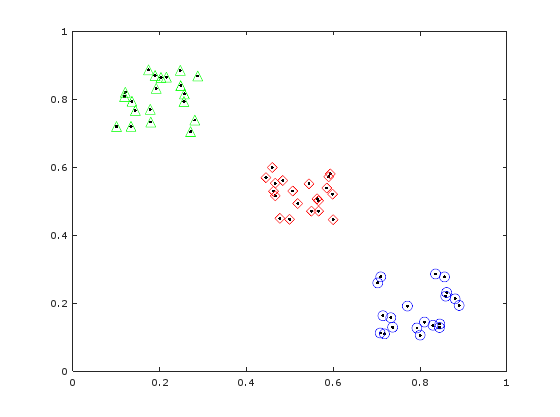
\includegraphics[width=0.45\textwidth]{kohonen.png}
  \caption{Clustered data using a SOM.}
  \label{fig:kohonen}
\end{figure}
\end{homeworkProblem}

\begin{homeworkProblem}
LVQ was quite difficult, as the number of neurons, the learning rate and decay parameters were tweaked until finding something.

{\large \textbf{Run details}}

The code \texttt{[w,acc] = lvq\_loop(data1, 5000)} yielded the following:
$$acc =  1 \quad
W = \begin{bmatrix}
0.462316 & 0.877874 \\
0.164309 & 0.793170 \\
-0.104877 & 0.489462 \\
0.465819 & -0.076281 \\
0.330399 & 0.435579 \\
0.155575 & 0.170246
\end{bmatrix}
$$
By using 6 neurons, that is, overfitted to the maximum.
However, 3 neurons were enough, with more training iterations.

\texttt{[w,acc] = lvq\_loop(data1, 5000)}:

$$acc =  1 \quad
w = \begin{bmatrix}
-0.091944 & 0.733631 \\
0.707465 & 0.011495 \\
0.238132 & 0.330761
\end{bmatrix}
$$
\end{homeworkProblem}

\begin{homeworkProblem}
The same story goes for problem 3, but instead using the \texttt{Iris} dataset.

The following parameters were used:

\begin{lstlisting}
>> [w,acc] = lvq_loop(data2, 1000)
lrate = 0.8;
decay = 0.05;
w =

   0.2229961   0.4159564   0.5371445   0.7452070
   0.6727481   0.9419399   0.4069340   0.0988960
   0.8154970   0.5843199   0.5376810   0.4165832
   0.7553312   0.3133215   0.7744005   0.4518696
   0.3642381   0.0749404   0.1702528   0.2977069
   0.6864519   0.5519802   0.7889211   0.6116886
   0.9809330   1.0312931   0.0545014   0.4077190
   0.1253019   0.3323812   0.0046333   0.6783671
   0.2664669   0.5714717   0.1522563   0.9543915
   0.7580878   0.9439515   0.7847167   0.9685561

acc =  1
\end{lstlisting}

It was also possible using even 3 neurons, given enough iterations.

\begin{lstlisting}
  >> [w,acc] = lvq_loop(data2, 1000)
  w =

     0.78196   0.86169   0.20912   0.24113
     0.66412   0.39710   0.99623   0.84333
     0.87452   0.28492   0.94403   0.58132

  acc =  1
\end{lstlisting}
\end{homeworkProblem}
\end{document}